\documentclass[11pt]{article}
\usepackage{setspace}
\setstretch{1}
\usepackage{amsmath,amssymb, amsthm}
\usepackage{graphicx}
\usepackage{bm}
\usepackage[hang, flushmargin]{footmisc}
\usepackage[colorlinks=true]{hyperref}
\usepackage[nameinlink]{cleveref}
\usepackage{footnotebackref}
\usepackage{url}
\usepackage{listings}
\usepackage[most]{tcolorbox}
\usepackage{inconsolata}
\usepackage[papersize={8.5in,11in}, margin=1in]{geometry}
\usepackage{float}
\usepackage{caption}
\usepackage{esint}
\usepackage{url}
\usepackage{enumitem}
\usepackage{subfig}
\usepackage{wasysym}
\newcommand{\ilc}{\texttt}
\usepackage{etoolbox}
\usepackage{algorithm}
\usepackage{changepage}
% \usepackage{algorithmic}
\usepackage[noend]{algpseudocode}
\usepackage{tikz}
\usetikzlibrary{matrix,positioning,arrows.meta,arrows}
\patchcmd{\thebibliography}{\section*{\refname}}{}{}{}
% \PassOptionsToPackage{hyphens}{url}\usepackage{hyperref}

\providecommand{\myceil}[1]{\left \lceil #1 \right \rceil }
\providecommand{\myfloor}[1]{\left \lfloor #1 \right \rfloor }


\begin{document}



\title{\textbf{CSDS 455: Homework 7}}

\author{Shaochen (Henry) ZHONG, \ilc{sxz517}}
\date{Due and submitted on 09/16/2020 \\ Fall 2020, Dr. Connamacher}
\maketitle

\section*{Problem 1}

\textit{I consulted \url{https://math.stackexchange.com/questions/666997/} for this problem.}\newline

With the Cayley's Formula (learned on Monday's class), we know that a $K_n$ graph will have $n^{n-2}$ spanning trees. We may create a bipartite graph with partitions $T, E$ where each node $t \in T$ represent a spanning tree of $K_n$, and each $e \in E$ represent an edge in $K_n$. Then we connect these two partitions if $e \in E(t)$.

It is known that each spanning tree of $K_n$ has $n-1$ edges, and we know that there are $n^{n-2}$ nodes $\in T$. Therefore the bipartite graph will have $(n-1) \cdot n^{n-2}$ edges. \newline

Due the nature of $K_n$, every edge of it is equivalent to another; this implies the number of spanning trees containing an edge will be the same as the number of spanning trees containing any other edge. Therefore each edge is contained by $\frac{(n-1) \cdot n^{n-2}}{{n \choose 2}} = 2n^{n-3}$ (as there are ${n \choose 2}$ edges in $K_n$). We substract this number from the total number of spanning tree of $K_n$, which is same as removing an edge $e$ from $K_n$, and there will be $ n^{n-2} - 2n^{n-3} = (n-2)n^{n-3}$ spanning tree left in $K_n - e$.

\section*{Problem 2}

There will be infinite number of classes. First it is easy to tell if edge $uv$ is not in the spanning tree, we may have two classes of spanning trees with the first class starts from $\chi u$, and the second from $\chi v$.\newline

However the interesting part is if $uv$ is contained in the spanning tree. For the ease of description let $d(uv) = 2m$, $d(u, \chi) = m + x$ ($x \geq 0$), and $y > 0$, we may have the below base cases:

\begin{figure}[H]
    \centering
    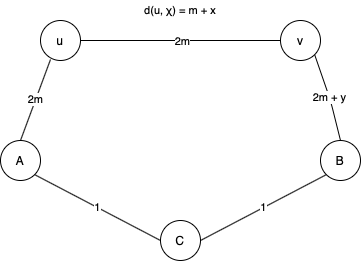
\includegraphics[width=0.45\linewidth]{{fig/fig_p2_1.png}}
    \label{fig:1}
\end{figure}

For $T_1$, assume $\chi$ is in the middle of $uv$ (which implies $x = 0$), in this case we shall have $d(\chi \rightarrow u \rightarrow A \rightarrow C) = m + 2m + 1 = 3m + 1$ and $d(\chi \rightarrow v \rightarrow B \rightarrow C) = m + 2m + y + 1 = 3m + y + 1$. So clearly we should connect $C$ to $A$, and we have $d_{T_1}(u, C) = 2m + 1$.

However, if we let $d(u, \chi) > d(v, \chi)$ on $uv$, to a point that $x > y$ in $T_2$. In this case we shall have $d(\chi \rightarrow u \rightarrow A \rightarrow C) = 3m + x + 1$ and $d(\chi \rightarrow v \rightarrow B \rightarrow C) = m - x + 2m + y + 1 = 3m - x + y + 1 < 3m + 1$. So we should connect $C$ to $B$, and $d_{T_2}(u, C) = 2m + 2m + y + 1 = 4m + 1 \neq d_{T_1}(u, C)$ \newline

\begin{figure}[H]
    \centering
    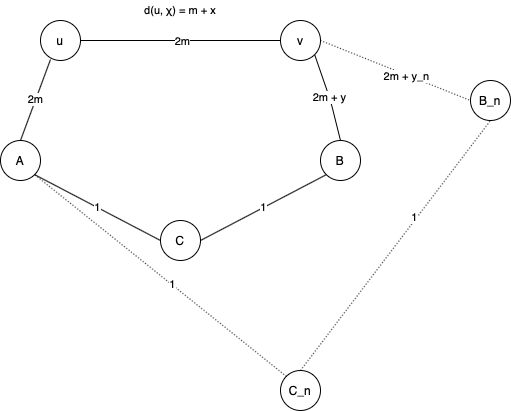
\includegraphics[width=0.7\linewidth]{{fig/fig_p2_2.png}}
    \label{fig:1}
\end{figure}

Since it is known that once this $x > y$ condition is established, the shortest path tree must detach $C$ from $A$ and connect it to $B$, this will make a new shortest path tree $T_n$ with $d_{T_n}(u, C) \neq d_{T_1}(u, c)$.

Note that we may have infinite edges like $vB$ and vertices like $C$; e.g. $vB_n$ and $C_n$, with a length of $d(v, B_n) = 2m + y_n$ , $d(B_n, C_n) = 1$, and $d(A, C_n) = 1$. And as we increase the value of $x$ on $d(u, \chi)$ (a.k.a moving $\chi$ passes midpoint of $uv$ and towards $v$ to make $\chi', \chi'',\chi''', ..., \chi_n$) to be $x_n$, we may find infinite pairs of $(x_n, y_n)$ where $x_n > y_n$, and thus we have infinite classes of non-equivalent spanning trees.\newline








% \section{References}
%
% \nocite{*}
% \raggedright
% \bibliography{references.bib}
% \bibliographystyle{plain}


\end{document}